% !TeX program = xelatex
% !TeX encoding = UTF-8 Unicode
% !BIB program = biber

\documentclass{relatorio}
\usepackage[hidelinks]{hyperref}
\cftsetindents{section}{1em}{3em}
\cftsetindents{subsection}{1em}{4em}
\usepackage{minted}
\usepackage{listings}
\usepackage{color}
\definecolor{lightgray}{rgb}{.9,.9,.9}
\definecolor{darkgray}{rgb}{.4,.4,.4}
\definecolor{purple}{rgb}{0.65, 0.12, 0.82}
\definecolor{applegreen}{rgb}{0.55, 0.71, 0.0}
\definecolor{azure(colorwheel)}{rgb}{0.0, 0.5, 1.0}
\definecolor{awesome}{rgb}{1.0, 0.13, 0.32}
\definecolor{ao(english)}{rgb}{0.0, 0.5, 0.0}
\definecolor{darkmidnightblue}{rgb}{0.0, 0.2, 0.4}

\lstdefinelanguage{cpp}{
	keywords={const, typeof, new, true, false, catch, function, return, null, catch, switch, var, if, in, while, do, else, case, break, long, int Reduced, Running, delta, debugging},
	keywordstyle=\color{blue}\bfseries,
	keywords=[2]{boolean, string, number, objectid},
	keywordstyle=[2]\color{green}\bfseries,
	identifierstyle=\color{darkgray},
	sensitive=false,
	comment=[l]{//},
	morecomment=[s]{/*}{*/},
	commentstyle=\color{purple}\ttfamily,
	stringstyle=\color{red}\ttfamily,
	morestring=[b]',
	morestring=[b]"
}

\lstset{language=cpp,
   extendedchars=true,
	basicstyle=\footnotesize\ttfamily,
	showstringspaces=false,
	showspaces=false,
	tabsize=2,
	breaklines=true,
	showtabs=false
}

\usepackage{parcolumns}
\usepackage{graphicx, subcaption}
\title{Is Software Debloating Useful? - A Comparative Study}
\addauthor{Sumit Lahiri}
\addauthor{Amit Kumar Sharma}
\setsubject{Analysis Study \& Comparision of Software Debloating Tools}
\preamble{}

\begin{document}
	
	\onecolumn
	\tableofcontents
	\twocolumn  
	% !TeX root = document.tex
% !TeX encoding = UTF-8 Unicode

\IEEEtitleabstractindextext{%
	\begin{abstract}
	In this course project we intend to understand, learn, run \& compare some \texttt{state-of-the-art} sofware debloating tools available for debloating large \texttt{C} or \texttt{C++} software project. In our quest to implement the project, we first started with a set of 3 motivating examples which showed where software deblaoting tools shine and why compiler optimization passes alone cannot do the task. 
	
	In short we modify, build and run software deblaoting tools on some benchmarks and see their performance in reducing or removing such code parts or instrcutions which may not be useful in the current context of using a particular tool. Knowing what all to remove from the code via automated debloating is a hard task since it will require through modelling of the environemnt and then making a call as to whether a certain piece of code will get executed or not. We can clearly see that it is not a trival problem to solve and thus, automated debloating is quite challenging. 
	
	We explore such tools that don't need a through execution environment modelling. These tools under exploration allow us to write a complete and sound specification of the desired properties or features that we want a given tool to be executable on thus eliminating the task of complex execution environment modelling. Now the problem is simplified and it boils down to removing all the undesired parts of the code that will never get executed in the current execution context. We refer to debloating as a iterative process by which these tools can now remove the undesired code sections from the source code or eliminate those instructions and function calls that will never be invoked making the final binary a sleek and trimmer down version instead of a bloated one. 
	
	We explore different techniques of software debloating and iterative reductions and see what works best under different functional requirements. Below is a comprehensive report of the work we did and our understanding of techniques adopted by each of the tools under exploration. 
	\end{abstract}
	
	\begin{IEEEkeywords}
		Software Debloating, Software Engineering, Delta Debugging, Reinforcement Learning, Markov Decision Process. 
	\end{IEEEkeywords}
}

	\maketitle{}

\section{Project Objective}%

We introduce and explain the issue involving \textbf{software bloating} that comes in given the nature and varied options 
available to develop modern software. We restrict ourselves to \texttt{C} or \texttt{C++} projects especially the once used frequently
as a part of \texttt{unix} or \texttt{darwin} oses. These projects are usually build and installed as standalone tools or as libraries 
for linking with other major tools. 

We propose to debloat a piece of \texttt{C or C++ Code} via \textbf{Policy Based Reinforcement Learning} using techniques and approaches as laid out in the two research papers we have selected for accomplishing the task. Both the papers have demonstrated novel techniques for debloating the codebase for a given \texttt{C or C++ Software} using \textbf{Policy Based Reinforcement Learning}, the \href{https://dl.acm.org/doi/10.1145/3243734.3243838}{first paper} mentioned does this by \textbf{Learning-Guided Delta Debugging}  while the \href{http://www.csl.sri.com/users/gehani/papers/MLSys-2019.DeepOCCAM.pdf}{second paper} does this by \textbf{Guided Function Specialization} technique. 

In our project \href{http://www.csl.sri.com/users/gehani/papers/MLSys-2019.DeepOCCAM.pdf}{(based out of Paper 2)}, we model the debloating problem as \textbf{reinforcement learning} where action would be to specialize a program or not. The state of the model will be a \textbf{vector} containing all the required details about the \textbf{specialized code}. The \textbf{reward} will be a \textbf{reduction} of the number of \textbf{instructions or code size} in the program after the program is debloated. As the model keeps learning, we expect the rewards to be improved with more inputs. 

Software deblaoting leads to reduction of attack surface and lesser code to build and install, given it is done meticulosuly. We use debloating 
techniques to perform debloating on these tools or library source code and report back the reductions we saw after debloating. As a part of the process
we get a deeper understanding of each of the tools and  how they function, modify them to get comparision metrics or implement them Eg. \texttt{DeepOCCAM} 
from research papers based on available source code. 

At the end we have a comprehensive report and working implementation of the modifiactions or runs we do to either in the benchamrks or in the tool's 
\texttt{source code} to suite the needs of the project. Given the limited time we got, not all things were completely implemented, especially the runs on other common
benchmarks would be needed for a clearer comparison of the tools. Nevertheless, we provide a comparison report based on the current runs and share our insghts on the suitability
of use of each tool in different contexts \texttt{(What technique works better than the other?)} 

\section{What is Software debloating?}%

$\textbf{Software bloating}$ is quite a common problem in any real world software project where the code base is plagued with LOCs that are not useful while the program runs in a given execution context, a common example being exposing too many $\textbf{redundant APIs}$, $\textbf{default configurations}$ for each context or many $\textbf{command line options}$ that are not used or never invoked in general but are still in the codebase. One primary reason for this is that it isn't possible to structure the code base before hand or to choose a strict design pattern for all components that we write. Many times code needs to be written on demand or ad-hoc basis because not all requirements are captured in the early stages of the project and that becomes the potential root cause for $\textbf{software bloating}$. $\textbf{Software bloating}$ can lead to bugs, slower code execution and even expose vulnerabilities in the code base. The current techniques used are $\textbf{manually thought}$ clever $\textbf{metrics \& heuristics}$ for identifying such $\textbf{bloat sites}$ and refactoring the code to remove them. 

\subsection{Software Debloating Tools}%

We focus on four popular tools we found for the purpose of software debloating of large scale \texttt{C or C++} projects, namely \texttt{Chisel}, \texttt{Trimmer}, \texttt{OCCAM} \& \texttt{DeepOCCAM} tools. These tools vary in the way they do debloating and the specifications needed in order to do effective and sound debloating. By effective and sound deblaoting, we are referring to thier capacity to reduce \texttt{function calls}, \texttt{instructions}, \texttt{direct loops} etc from the original source code and produce a binary that is best suited to a given runtime 
environment context with out hampering the normal \texttt{desired} execution of the program. On different \texttt{environemnts}, based on the specifications we give and the way the binary is executed, the exact debloating effect of \texttt{reductions} may be differ significantly since the \texttt{desired} property specification may vary based on the \texttt{OSes} we run them on or the \texttt{settings/parameters} needed for normal run. 

In each of these tools, we need to provide some information in the form of \texttt{desired} properties that we want our final program to meet under all safe condition and remove the other parts of the \texttt{code} or \texttt{instructions} that we dont need in the current execution context of the final binary produced.  

\subsection{Software Debloating Techniques}%

The techniques used by these tools for effective debloating varies from tool to tool but the the overall nature of the transformation can be catagorized into two types \texttt{source-to-source} \& \texttt{source-to-binary} transformation. 

In \texttt{source-to-source} transformation the tool's input is the bloated \texttt{source code} and the \texttt{specification} in the form of tests that need to pass under a given execution environment. The tool produces a \texttt{debloated} source code and binary from the input \textbf{source}. This is usually guided by a machine learning model and the reduction happens via techniques similar to \texttt{dead code elimination}. Some examples of tools running like this are \texttt{Chisel} \& \texttt{Razor}
 
In \texttt{source-to-binary} transformation the tool's input is the bloated \texttt{source code} and the \texttt{specification} listing statically known arguments to the \texttt{main()} function and other \texttt{dynamic arguments} needed under a given execution environment. The tool produces a \texttt{debloated} binary from the input \textbf{source} but doesnot produce \texttt{debloated source code} unlike the technique mentioned above. 

This is usually guided by hand crafted heuristics for \texttt{function specialization} at each \texttt{call-site} and the reduction happens via techniques similar to \texttt{dead code elimination} or other \texttt{compiler optimization} passes. Some examples of tools running like this are \texttt{Trimmer} \& \texttt{OCCAM} but the exact algorithms for \texttt{constant propagation}, \texttt{function specialization} \& \texttt{function inlining} differs in both the tools. 

Another approach for \texttt{function specialization} at each \texttt{call-site} is by using machine learning to decide as to \texttt{when to specialize} and then do regular reduction in a similar fashion as above. \texttt{DeepOCCAM} is an example of this technique. 

\section{Motivating Examples}%

As a motivating example we show what current \texttt{compiler optimization} techniques fail to do and \textbf{why} special software deblaoting tools are needed for the purpose of \texttt{debloating}, we here show the working of the \texttt{Chisel} tool since \texttt{source-to-source} transforamtion is of \texttt{particular interest} to most software developers. We show the \texttt{original} source code

\begin{lstlisting}
#include <stdio.h>
void run(int a) {
	if (a > 90) {
		printf("%d\n", a);
	}
}
long long int add(int a, int b) 
{ return a + b; }
long long int sub(int a, int b) 
{ return a - b; }
int main(int argc, char *argv[]) {
	int c = 0;
	c = -500;
	if (c > 0) {
		run(c);
		add(c, c + 1);
	} else {
		sub(c + 90, c);
	}
	return 0;
}
\end{lstlisting} 

and the \texttt{chiseled} source code below it on a \textbf\texttt{blank test} case where nothing is \texttt{desirable} in the code. 

\begin{lstlisting}
	#include <stdio.h>
	int main(int argc, char *argv[]) {
		int c = 0;
		return 0;
	}
\end{lstlisting}

We were amazed at the amount by which \texttt{Chisel} was able to reduce the source code via \texttt{reinforcement guided delta-debugging} on this \textbf\texttt{blank test} case. We now show what \texttt{gcc} with \texttt{-O3} optimization was able to do with the code. This is acceptable since the \textbf{gcc compiler} has no way to remove the code directly based on current techniques of \texttt{code optimization} and thus \texttt{debloaters} to the rescue. 

\begin{figure*}
	\centering
	\captionsetup{justification=centering}
	\includegraphics[width=1\linewidth]{imgs/chisel_before.png}
	\caption{\textbf{\texttt{C Code}} Example \color{red} before \color{black} \textbf{Chisel} tool processing on \texttt{blank test} case}%
	\label{fig:plant}
	\centering
	\captionsetup{justification=centering}
	\includegraphics[width=1\linewidth]{imgs/chisel_after.png}
	\caption{\textbf{\texttt{C Code}} Example \color{green} after \color{black} \textbf{Chisel} tool processing on \texttt{blank test} case}%
	\label{fig:plant}
\end{figure*}

We now show \texttt{Chisel} tool in action.
 
\begin{lstlisting}
Start global reduction
Running delta debugging - Size: 3
Start local reduction
Reduce process_aflag at test.c
Running delta debugging - Size: 1
Reduced - Size: 0
Reduce process_bflag at test.c
Running delta debugging - Size: 2
Reduced - Size: 1
Reduced - Size: 0
Reduce process_cflag at test.c
Running delta debugging - Size: 3
Reduced - Size: 1
Reduced - Size: 0
Reduce main at test.c
Running delta debugging - Size: 2
Reduced - Size: 1
Iteration 2 (Word: 58)
Start global reduction
Running delta debugging - Size: 3
Reduced - Size: 1
Reduced - Size: 0
Start local reduction
Reduce main at test.c
Running delta debugging - Size: 1
Iteration 3 (Word: 43)
Start global reduction
Running delta debugging - Size: 0
Start local reduction
Reduce main at test.c
Running delta debugging - Size: 1
Reduce File: test.c
Iteration 1 (Word: 43)
Start global reduction
Running delta debugging - Size: 0
Start local reduction
Reduce main at test.c
Running delta debugging - Size: 1
\end{lstlisting}

We now show a working of the \texttt{OCCAM} tool on a different \texttt{getopt()} based \texttt{C} example. We pass in some default static arguments to the program and see the \texttt{OCCAM} tool in action on it.

We present the \texttt{static analysis} details for \texttt{OCCAM} run in \color{red} before \color{black} \&
\color{green} after \color{black} all \texttt{inter} \& \texttt{intra} specialization passes have been completed. The example \texttt{C} code is as below. It accepts \texttt{three flags} namely \texttt{-a}, \texttt{-b} \& \texttt{-c} and call a function based on the \texttt{flag} recieved.

\begin{lstlisting}
#include <stdio.h>
#include <stdlib.h>

void process_aflag(int a) 
{ printf("%d\n", a + 90); }
	
void process_bflag(int a) {
	a = 80 * a;
	process_aflag(a);
}

void process_cflag(int a) {
	a = a << 20;
	process_aflag(a);
	process_bflag(a);
}
// Example based on : http://osr507doc.sco.com/en/tools/ccs_stdio_args.html
int main(int argc, char *argv[]) {
	/* Function flags */
	int aflag = 0;
	int bflag = 0;
	int cflag = 0;
	int ch;
	
while ((ch = getopt(argc, argv, "abc")) != -1) {
	/* For options present */
	/* set flag to some value */
	/* else write out an error statement */		
	switch (ch) {
		case 'a':
			aflag = 10;
			fprintf(stdout, "aflag set !\n");
			process_aflag(aflag);
			break;
		case 'b':
			bflag = 20;
			fprintf(stdout, "bflag set !\n");
			process_bflag(bflag);
			break;
		case 'c':
			cflag = 30;
			fprintf(stdout, "cflag set !\n");
			process_cflag(cflag);
			break;
		default:
			(void)fprintf(stderr, "Usage: %s [-abc]\n", argv[0]);
			return (2);
		}
	}
	if (aflag < 0) {
		process_cflag(90);
	}
	/* Do other processing controlled by aflag, bflag, cflag. */
	process_bflag(60)
	return (0);
}
\end{lstlisting} 

The \texttt{Manifest file} we used for running \texttt{OCCAM} in \texttt{aggressive mode}  

\begin{lstlisting}
{ "main" : "test.o.bc"
, "binary"  : "test"
, "modules"    : []
, "native_libs" : []
, "static_args"    : ["-a", "90"]
, "name"    : "test"
}
\end{lstlisting} 

\texttt{OCCAM} log after run was complete. We see that there was reduction of the code size that was finally complied to binary. 

\begin{lstlisting}
Statistics for  before specialization
[CFG analysis]
4 	Number of functions
0 	Number of specialized functions
0 	Number of bounced functions added by devirt
15 	Number of basic blocks
81 	Number of instructions
13 	Number of direct calls
6 	Number of external calls
0 	Number of assembly calls
0 	Number of indirect calls
0 	Number of unknown calls
1 	Number of loops   
0 	Number of bounded loops
[Memory analysis]
37 	Number of memory instructions
32 	Statically safe memory accesses
5 	Statically unknown memory accesses

Statistics for  after specialization
[CFG analysis]
4 	Number of functions
0 	Number of specialized functions
0 	Number of bounced functions added by devirt
15	Number of basic blocks
60 	Number of instructions
13 	Number of direct calls
7 	Number of external calls
0 	Number of assembly calls
0 	Number of indirect calls
0 	Number of unknown calls
1 	Number of loops   
0 	Number of bounded loops
[Memory analysis]
19 	Number of memory instructions
15 	Statically safe memory accesses
4 	Statically unknown memory accesses
\end{lstlisting} 

\section{OCCAM Tool}%
\label{Tools}

OCCAM is a debloating tool that works on the principle of winnowing and object culling. Winnowing is a static analysis and code specialization technique based on the partial evaluation algorithm. It is a code optimization technique where all the static inputs computations are processed during compile time. Also, all the function arguments 
are replaced with constant value (if statically known) and optimization passes by LLVM is applied after that. PE helps to achieve the residual program which runs faster than the original program with reduction in gadgets and instruction count. 

\subsection{Overview}%
\label{Tools}

We detail out a bit more about the OCCAM tool here. Function inlining only replaces the function call by the function definition but PE takes an extra step and evaluates the function before the execution of program using statically known arguments via constant folding or constant propagation in the function body. Static (compile time) analysis is seperate from dynamic (run time) analysis with this algorithm 
and thus we present details of the tool runs in two sections Static Analysis and Dynamic Analysis.

Partial evaluation works in two steps: (a) Optimization (b) Specialization
In optimization phase compile time constants are identified, dead codes are eliminated and the control flow of the program is reduced. In specialization phase, program is effectively specialized across function boundaries.

OCCAM takes two inputs: a source code in C/C++ and a manifest file in JSON format. The debloated binary of the original source code produced by the OCCAM tool 
is used by the Gadget set Analyser to get the gadgets count. The original source code is also compiled by a compiler and feed to GSA tool. Both debloated and original binaries are then compared for reduction in metric counts. Dead code elimination in OCCAM works in five ways:
\\
•	Aggressive Non-Recursive DCE.
\\
•	Inter Procedural DCE.
(accross function calls) \\
•	Intra Procedural DCE.
(for basic blocks in function body) \\
•	Sparse Conditional Constant Propagation based DCE.
(for Trimmer, we enable this pass) \\
•	Abstract Interpretation based DCE. (Seahorn Crab based DCE pass) \\

\subsection{Working Procedure}%
\label{Tools}

Program debloating techniques. Program deblaoting techniques rogram debloating techniques. Program deblaoting techniques
rogram debloating techniques. Program deblaoting techniquesrogram debloating techniques. Program deblaoting techniques
rogram debloating techniques. Program deblaoting techniques rogram debloating techniques. Program deblaoting techniques
rogram debloating techniques. Program deblaoting techniques 
rogram debloating techniques. Program deblaoting techniquesrogram debloating techniques. Program deblaoting techniques
rogram debloating techniques. Program deblaoting techniques

\section{Trimmer Tool}%
\label{Tools}

Program debloating techniques. Program deblaoting techniques rogram debloating techniques. Program deblaoting techniques
rogram debloating techniques. Program deblaoting techniquesrogram debloating techniques. Program deblaoting techniques
rogram debloating techniques. Program deblaoting techniques rogram debloating techniques. Program deblaoting techniques
rogram debloating techniques. Program deblaoting techniques 
rogram debloating techniques. Program deblaoting techniquesrogram debloating techniques. Program deblaoting techniques
rogram debloating techniques. Program deblaoting techniques

\subsection{Overview}%
\label{Tools}

TRIMMER tool is used to specialize the target program with respect to the user defined configuration. The configuration contains the usage context of application. Compiler transformation are included in this tool for good debloating.Inter procedural  constant propagation is used in the tool which aggressively removes the unnecessary codes. With the reduction in the unused program codes, the gadget count of the program is also reduced and helps to improve the security performance of the system. 

\subsection{Working Procedure}%
\label{Tools}

The source code is converted to LLVM IR  and given as an input to the trimmer tool along with the manifest file consisting of user defined configuration. The TRIMMER first performs input specialization with respect to the user defined configuration . The second part is loop unrolling . The loop unrolling becomes important step to make interprocedural constant propagation easier. Constant Propagation is the final stage in the tool. The specialized code processed by the TRIMMER is then given as input to the linker . The linker also reads the linker flags from the manifest file and generates a final specialized binary executable file.

\section{Chisel Tool}%
\label{Tools}

We share a brief information about the tool. \textbf{Chisel} tool works by learning a \textbf{policy} for \textbf{delta debugging} by \textbf{reinforcement learning} which guarantees \textbf{1-minimal P*} \& $\textbf{$O(|P|^2)$}$ runtime. The abstraction is that a \textbf{markov decision process} is being used to model the \textbf{reinforcement learning} problem for meaningful \textbf{guidance} to learn the \textbf{policy} in a better way. All global declarations, variables, functions etc. are first reduced by the delta-debugging principle as state above and thereafter local variables, loop declarations and arguments to functions are optimized. After both the local and global level reductions are done, \textbf{Chisel} invokes a run of the \textbf{global level reduction} again and repeats the process continually until the \textbf{1-minimal P*} version of the program is found. 

\subsection{Overview}%
\label{Tools}

\textbf{Chisel} tool's working is based on syntax guided hierarchical delta debugging algorithm. The tool ensures that the reduced program are compilable, core functionalities of source program are preserved  and undefined behaviours for non core functionalities does not show up. CHISEL also keeps all the criteria required for the system to work properly in order. The criteria are minimality,naturalness,efficiency,robustness and generality. The probabilistic model is used in CHISEL to accelerate the delta debugging algorithm and Markov Decision Process is used to search a proper policy for learning the machine learning algorithm. Model based Reinforcement algorithm is used to converge to the solution quickly.

\subsection{Working Procedure}%
\label{Tools}

The input to the \textbf{CHISEL} tool is a C/C++ source file (test.c) which is to be debloated. Along with the source file , we give a specialized script which contains the high level specification of the desired output. The CHISEL tool then generates binary of the source code(test.c.chisel.c). Both the source and debloated program are then compiled by g++ or any other compiler and the binaries generated by the compiler are given to the ROP gadgets or Gadget Set Analyser(GSA) . The ROP gadget outputs the count of the  gadgets before and after debloating respectively.

\subsection{State Encoding}%
\label{Tools}

Markov Decision Process is used for Delta debugging algorithm. For  delta debugging algorithm two things are required and the tuple of these two things defines the state of the model at any time. The first thing is the pair of the program to be tested and second thing is the number of partitions into which a program is broken. The initial state consist the entire program  represented as a list into two partitions. The program can be broken inti tokens,identifiers ,statements or even a finer granularity is reached to obtain the minimal state.

\subsection{Delta Debugging}%
\label{Tools}

Delta debugging is an algorithm or technique to remove the unnecessary part of the input which is not responsible for test case failure. DD makes testing easier as it divides input into smaller subsets because smaller  and simplified testcases are easy to handle. Delta debugging algorithm is used till we reach 1-minimal expression. DD is an iterative algorithm.Markov Decision Process for delta debugging is deployed to build a statistical model to get 1-minimal solution with lesser number of iterations than delta debugging alone.


\subsection{1-minimal Program}%
\label{Tools}

Suppose we have a testcase T which fails the program P. When T is given as input to P, the entire part of T may not be responsible for causing failure to the program P. Therefore, we are interested in the exact part of T which causes the program to fail. In short, we can say failing test case can have relevant and non-relevant information. To filter out the relevant information from the test case, we use Delta debugging algorithm.If a test case T fails the program P, then the expression T’ derived from T is 1-minimal iff any deviation causes the test case failure to go away.

	\begin{figure}[H]
	\centering
	\captionsetup{justification=centering}
	\includegraphics[width=0.65\linewidth]{imgs/chisel_learning_mkdir_plot.png}
	\caption{Learning plot for \color{blue} mkdir}%
	\label{fig:plant}
	\centering
	\captionsetup{justification=centering}
	\includegraphics[width=0.65\linewidth]{imgs/chisel_learning_date_plot.png}
	\caption{Learning plot for \color{blue} date}%
	\label{fig:plant}
	\centering
	\captionsetup{justification=centering}
	\includegraphics[width=0.65\linewidth]{imgs/chisel_learning_chmown-main_plot.png}
	\caption{Learning plot for \color{blue} chown}%
	\label{fig:plant}
	\centering
	\captionsetup{justification=centering}
	\includegraphics[width=0.65\linewidth]{imgs/chisel_learning_bzip2_plot.png}
	\caption{Learning plot for \color{blue} bzip2}%
	\label{fig:plant}
	\centering
	\captionsetup{justification=centering}
	\includegraphics[width=0.65\linewidth]{imgs/chisel_gadgets_yyparse_plot.png}
	\caption{Gadgets plot for \color{blue} yyparse}%
	\label{fig:plant}
\end{figure}
\begin{figure}[H]
	\centering
	\captionsetup{justification=centering}
	\includegraphics[width=0.65\linewidth]{imgs/chisel_gadgets_mkdir_plot.png}
	\caption{Gadgets plot for \color{blue} mkdir}%
	\label{fig:plant}
	\centering
	\captionsetup{justification=centering}
	\includegraphics[width=0.65\linewidth]{imgs/chisel_gadgets_date_plot.png}
	\caption{Gadgets plot for \color{blue} date}%
	\label{fig:plant}
	\centering
	\captionsetup{justification=centering}
	\includegraphics[width=0.65\linewidth]{imgs/chisel_gadgets_chmown-main_plot.png}
	\caption{Gadgets plot for \color{blue} chown}%
	\label{fig:plant}
	\centering
	\captionsetup{justification=centering}
	\includegraphics[width=0.65\linewidth]{imgs/chisel_gadgets_bzip2_plot.png}
	\caption{Gadgets plot for \color{blue} bzip2}%
	\label{fig:plant}
	\centering
	\captionsetup{justification=centering}
	\includegraphics[width=0.65\linewidth]{imgs/chisel_gadgets_yyparse_plot.png}
	\caption{Gadgets plot for \color{blue} yyparse}%
	\label{fig:plant}
\end{figure}

\section{DeepOCCAM Tool}%
\label{Tools}

Deepoccam is an extension of occam tool with new approach based on machine learning. Both occam and Deepoccam are based on the partial evaluation approach.
The major contribution of PE is to determine if the function specialization decreases the size of residual program. The function specialization increases the code
size of original program but then optimization in the new function  such as constant propagation can be possible after function inlining and static values substitution.
So, there is an opportunity for code size reduction in the residual program after partial evaluation process. 

\subsection{Overview}%
\label{Tools}

Whether or not the function specialization reduces the code size is not trivial. 
This is the problem with occam as it implements "never specialize" or "always specialize" approaches only. So, it becomes important that we come up an automatied approach to learn 
when to specialize. The machine learning model can be considered as a better approach which has been implemented in DeepOCCAM. The specialization depends on the present state of the program 
and does not consider the past changes made to the program. It follows Markov Decision process. Reinforcement Learning seems to a best fit for this approach where the rewards are reduction 
in metrics value under consideration. So, DeepOCCAM is implemented with policy-learning based RL model where the rewards are dynamically evaluated and the actions depend on the current encoded state 
and the metric values.

\subsection{Working Procedure}%
\label{Tools}

Program debloating techniques. Program deblaoting techniques rogram debloating techniques. Program deblaoting techniques
rogram debloating techniques. Program deblaoting techniquesrogram debloating techniques. Program deblaoting techniques
rogram debloating techniques. Program deblaoting techniques rogram debloating techniques. Program deblaoting techniques
rogram debloating techniques. Program deblaoting techniques 
rogram debloating techniques. Program deblaoting techniquesrogram debloating techniques. Program deblaoting techniques
rogram debloating techniques. Program deblaoting techniques

\subsection{State Encoding}%
\label{Tools}

	State Encoding:
Deepoccam have been implemented with two state models:
1. Handcrafted features
2.LLVM IR embeddings Inst2vec

In HF, the state contains the details about the caller,callee, compilation unit and call site. The state in this case is a combination of these four features vectors.

In Inst2vec each instruction is converted to a vector using skip gram model . The LLVM IR of the caller,calle and calling context is represented as a list of instructions. 
Also the arguments at the call site is represented as a bit vector of 0 \& 1 where Zero(0) denotes unknown arguments and one(1) denotes the statically known arguments.
This bitvector alongf with the above three vectors form a tuple of the four 2-D matrices. These tuple represents the state for the RL model. 


\subsection{Inst2Vec Usage}%
\label{Tools}

Inst2vec  is the technique of processing the source code into the features vector for modeling the Reinforcement Learning. It follows an approach similar to skip-gram model in Natural Language Processing of pre-defined context size. The source code is first compiled into LLVM IR code. The LLVM IR is in the form of a static single assignment.As LLVM IR  is independent of machine or hardware architecture and programming language , it becomes easy to train the program embeddings.The approach is similar to word2vec model.


With the LLVM IR , the contextual flow graph (XFG)is created. XFG takes into account both the data flow and control flow of the program. With these XFGs generated from LLVM IR , the consecutive statement pairs are made of pre-defined context size . These statement pairs are then  checked for duplication. The XFGs pairs are made by constructing a dual graph with statement as nodes and removing duplicate edges. The process is then followed by removing statements of negligible presence. We get an inst2vec after subsampling of frequent pairs which can be optimized and trained. XFGs ensures that the semantics of statements are preserved.

\section{Project Aim}%
\label{Tools}

As a experimental \& comparison based project, our task was to run the tools on various examples to see for \texttt{static} 
\& \texttt{dynamic} metric changes \textbf{before} \& \textbf{after} the run of the tools on these examples. 
We setup up each tools and prepare them for metrics that we want to extract \& compare in each of the runs using either 
statistics that are shown by the tool itself using options like \texttt{--stats} or \texttt{--opt-stats} for static analysis case 
or generating intermediate \texttt{binary} or \texttt{elf-section object} files for dynamic analysis.

We finally report an \textbf{overview}, \textbf{setup}, \textbf{benchmarks} \& \textbf{comparision} of these tools on some same 
examples and also on a set of \texttt{benchmarks} used originally to test run each of the tools in the original papers. 

We also implement a modification of \texttt{OCCAM} tool to run like \texttt{Trimmer} tool as per description and our understanding 
of the \textbf{Trimmer} original paper and a modification of base \texttt{OCCAM} tool to \texttt{DeepOCCAM} which uses a 
\texttt{reinforcement learning} based approach to specialization based on \textbf{DeepOCCAM} paper. 

\section{Implementation Overview}%
\label{Tools}

We elaborate on the changes and the work we did to meet the \texttt{Project Aim}. We start with the \texttt{Chisel} tool where we did modifications to dump the reduced chunk and the original chunk sizes that are used for \texttt{markov decision} based \texttt{delta-debugging} and used it as a metric to measure the \texttt{learning rate} along with reduction in \texttt{gadgets} count for the intermediate binary produced by \texttt{Chisel} tool

For \textbf{OCCAM} tool the modification was to fix the code for running in our environment and then work on the \texttt{manifest} \& \texttt{automated} make builds so that it can be run in \texttt{dockers} for final release in the project. Another modification was to dump the \texttt{counts} for \texttt{caller}, \texttt{callee}, \texttt{constant arguments}, \texttt{statically known arguments} and other \texttt{context} related details for 
\texttt{metadata} \& \texttt{dataset} generation in the base \texttt{occam.log} file itself since \textbf{we were not able to complete the \texttt{gRPC} implementation on time} owing to build and linking related issues. 

For \textbf{DeepOCCAM}, we found a \textbf{\href{https://github.com/nhamlv-55/OCCAM/tree/mlpolicy}{half-implemented code}} repository which belongs to one of the authors for \textbf{DeepOCCAM} paper. The tool doesn't link, build or run on the current platform that we are using. It gave us insights on implementing some of the parts in the code that we are developing as an extension on \textbf{OCCAM} to develop \textbf{DeepOCCAM}.

The benchmarks we used needed modification interms of running it against updated \textbf{\href{https://github.com/SRI-CSL/gllvm}{gllvm}}, \textbf{\href{https://github.com/SRI-CSL/whole-program-llvm}{wllvm}} \& \textbf{\href{https://github.com/lahiri-phdworks/llvm-project/tree/release/10.x}{llvm-10}}. There were a few other tools and frameworks that we had to install and test in-order to run the debloating tools on these benchamarks. 

We compiled, build \& ran the tools in \texttt{docker} containers interacting with the base \texttt{OS} via \texttt{docker volumes} \& \texttt{u-tty terminal} program.

\section{Pipeline Setup}%
\label{Tools}

We divided the task of running the \texttt{benchmark} \& \texttt{motivating} examples for the \texttt{three} tools into \texttt{three} different \texttt{pipelines}. Each \texttt{pipeline} was built and deployed against different \texttt{Ubuntu OS} base \texttt{images} which was specifically required for \texttt{each} of the tools. There were some \texttt{libraries}, \texttt{python packages} and linking \texttt{object files} that conflicted when trying to run all three tools in the current base \texttt{OS} on which we were developing the tools, so we switched to using three \texttt{docker} containers one for each \texttt{tool} 

We ran multiple instances of the \texttt{docker} containers for \texttt{training} and \texttt{parellel} benchmark runs so that we can cover as many as \texttt{benchmark} code examples possible. We now show \texttt{architecture} diagrams of the final \texttt{pipelines} that we intend to use for \texttt{demonstration} purposes. 

\onecolumn
\begin{figure}[H]
	\centering
	\captionsetup{justification=centering}
	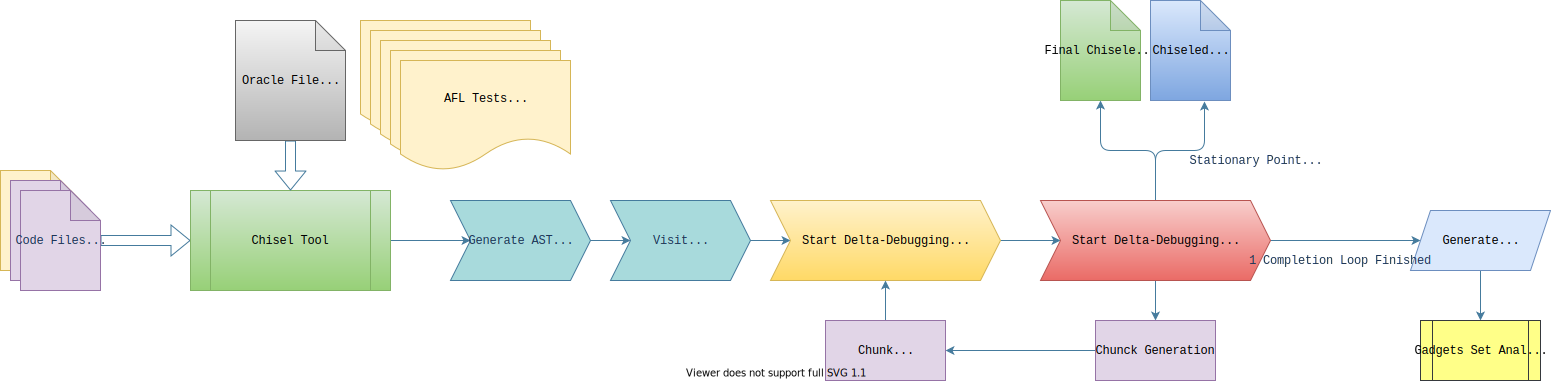
\includegraphics[width=1\linewidth]{imgs/chisel-pipeline.png}
	\caption{\textbf{Chisel Pipeline} : Setup \texttt{Chisel} runs on \texttt{Chisel-Benchmarks} \& other examples}%
	\label{fig:plant}
	\centering
	\captionsetup{justification=centering}
	\includegraphics[width=1\linewidth]{imgs/occam-pipeline.png}
	\caption{\textbf{OCCAM Pipeline} : Setup \texttt{OCCAM} runs on \texttt{OCCAM-Benchmarks} \& other examples}%
	\label{fig:plant}
	\centering
	\captionsetup{justification=centering}
	\includegraphics[width=1\linewidth]{imgs/occam-modified-trimmer.png}
	\caption{\textbf{Trimmer Runs} : Setup \texttt{Trimmer} runs on \texttt{OCCAM-Benchmarks} only}%
	\label{fig:plant}
\end{figure}
\twocolumn

\subsection{Chisel Pipeline}%
\label{Tools}

We give an overview of what we modified and how we setup the dockers for running the Chisel Tool. The markov model  code implementation in Chisel tool is in ProbabilisticModel.cpp where we added a function to dump a few heuristics.
We modified the GlobalReduction.cpp \& LocalReduction.cpp code files to dump the before and after chunk sizes for plotting the learning rates. After the .reduced binary produced at each stage when the tests as per \texttt{crash\_inputs} from AFL were executed, we run a \texttt{single\_run()} function of the modified GadgetSetAnalyzer to get the gadgets metric counts and plot them via matplotlib. We installed all dependencies of Chisel and cloned the modified GitHub repository for the runs in a docker container running debian:buster image. We dump the plots from the data collected after the final bianry is produced. The benchmarks already contained the AFL \texttt{crash\_inputs} and other tests, so we used them directly in our runs. 

\subsection{OCCAM Pipeline}%
\label{Tools}

We prepare the benchmarks for the OCCAM run. We modfied and rewrote many of the Makefiles and manifests for proper running of the benchmark examples. Some of the benchmark runs failed for OCCAM amalgamation (pass to combine all the bitcode files) and we only produced the static analysis metrics for these benchmark sets. We were able to run OCCAM for the portfolio benchmark runs used in the Trimmer paper published. We ran the scripts for OCCAM using different settings like --none, --onlyonce, --aggressive, --nonrec-aggressive for both --inter-spec and --intra-spec policy and dumped the metrics accordingly for each run. 

The docker base image used for the OCCAM is ubuntu:bionic. We installed all the dependencies and other tools like 
wllvm, gllvm, golang, llvm-10 etc for the runs. slash is the command line tool name for the python package razor that is uses the occam libraries and binary for debloating action. razor package is wrapper around the occam binary which runs the appropriate passes in occam via llvm-opt tool. It links and runs the tool against the source code and the manifest file supplied. 

We collect the data for each run of the benchmark for the different options of run available in the slash tool against the occam binary. We cloned the modified repository for OCCAM, built it from source and then ran the slash tool after the build via Makefiles and bash scripts (build.sh). We show a sample of the same below. 

\subsection{Trimmer Runs : OCCAM-T}%
\label{Tools}

We didn't have the source code to Trimmer, so we modified OCCAM code to run with argument specialization, LLVM loop unrolling and sparse conditional constant propagation. 
We make a docker container from the base OCCAM-pipeline docker image of the above. It already has all the tools and libaries needed for the build after the modifications we did to OCCAM source code. We added a LLVM opt pass for bounded loop unrolling, added the LLVM pass for IPSCCP implemeted in LLVM and set all the specialization decisions to true if an argument is constant specializable similar to the case of OCCAM running with Aggressive Poliy for inter and intra specialization passes over each function call sites. 

Simalar to OCCAM, we ran the modified benchmark scripts using --ipdse (for -Pipsccp), --unroll-loop (in passes.py in razor) and dumped along with LLVM the metrics accordingly for each run. The green column in the static analysis tables in for OCCAM-T (we call this modification to OCCAM as OCCAM-T instead of Trimmer).

A word on \textbf{Trimmer}, \textbf{OCCAM} also uses partial evaluation concept like \textbf{Trimmer} for specializing functions at call-sites but it is less aggressive compared to the  \textbf{Trimmer} because it does not include \textbf{\texttt{specialized loop unrolling}} and the modified \textbf{\texttt{constant propagation}} implementation in Trimmer Tool

\subsection{DeepOCCAM Pipeline}%
\label{Tools}

We found a \textbf{\href{https://github.com/nhamlv-55/OCCAM/tree/mlpolicy}{half-implemented code}} repository which belongs to one of the authors for \textbf{DeepOCCAM} paper. The tool doesn't link, build or run on the current platform that we are using. It gave us insights on implementing some of the parts in the code that we are developing as an extension on \textbf{OCCAM} to develop \textbf{DeepOCCAM}.

\begin{itemize}
	\item Modified code in base \textbf{OCCAM} tool to collect \textbf{RL} related features in the \texttt{occam.log} file. 
	\item Implemented a \textbf{deep reinforcement learning model} from the insights we got from the \textbf{\href{https://github.com/nhamlv-55/OCCAM/tree/mlpolicy}{half-implemented code}}. We were stuck on how to do the rewards implementation and the above repository helped us in implementating the same. 
	\item We setup a \textbf{docker} based container pipeline to build, run and debloat an example \textbf{\color{blue} code repository}. The \textbf{training} part happened outside the docker, we just saved and extracted the model for later use in container. 
	\item We had to modify the way the tool was plotting and processing some the feature vectors. We used \textbf{\texttt{Adam Optimization}}, \textbf{\texttt{ReLU}} functions, \textbf{\texttt{Softmax}}, \textbf{\texttt{torch.nn GRU}} neural net for \textbf{\texttt{inst2vec}} \& \textbf{\texttt{Linear fully-connected}} layers etc. for implementing the \textbf{\texttt{ML}} part of \textbf{DeepOCCAM} tool. 
\end{itemize}

\onecolumn
\begin{figure}[H]
	\centering
	\captionsetup{justification=centering}
	\includegraphics[width=0.83\linewidth]{imgs/deepoccam-pipeline.png}
	\caption{\textbf{DeepOCCAM Pipeline}}%
	\label{fig:plant}
	\centering
	\captionsetup{justification=centering}
	\includegraphics[width=0.83\linewidth]{imgs/deepoccam-pipeline.png}
	\caption{\textbf{DeepOCCAM : Based on Paper}}%
	\label{fig:plant}
\end{figure}
\twocolumn

\begin{figure}[H]
	\centering
	\captionsetup{justification=centering}
	\includegraphics[width=1\linewidth]{imgs/deepoccam_HF_learning_bzip_TOTAL_plot.png}
	\caption{\textbf{DeepOCCAM} \textbf{Total} \\ \textbf{450} iterations \color{blue} bzip - HF}%
	\label{fig:plant}
	\centering
	\captionsetup{justification=centering}
	\includegraphics[width=1\linewidth]{imgs/deepoccam_inst2vec_bzip_Total_plot.png}
	\caption{\textbf{DeepOCCAM} \textbf{Total} \\ \textbf{300} iterations \color{blue} bzip - inst2vec bzip embedding}%
	\label{fig:plant}
	\centering
	\captionsetup{justification=centering}
	\includegraphics[width=1\linewidth]{imgs/plots/chisel_learning_bzip-main_plot.png}
	\caption{\textbf{Chisel} Learning bzip \textbf{\texttt{main()}}}%
	\label{fig:plant}
\end{figure}
\begin{figure}[H]
	\centering
	\captionsetup{justification=centering}
	\includegraphics[width=1\linewidth]{imgs/plots/deepoccam_HF_bzip_JOP_plot.png}
	\caption{\textbf{DeepOCCAM} \textbf{JOP} \\ \textbf{400} iterations \color{blue} bzip - HF}%
	\label{fig:plant}
	\centering
	\captionsetup{justification=centering}
	\includegraphics[width=1\linewidth]{imgs/plots/deepoccam_inst2vec_bzip_JOP_plot.png}
	\caption{\textbf{DeepOCCAM} \textbf{JOP} \\ \textbf{300} iterations \color{blue} bzip - inst2vec bzip embedding}%
	\label{fig:plant}
	\centering
	\captionsetup{justification=centering}
	\includegraphics[width=1\linewidth]{imgs/plots/chisel_gadgets_bzip-main_plot.png}
	\caption{\textbf{Chisel} Gadgets Count \textbf{\texttt{main()}}}%
	\label{fig:plant}
\end{figure}

\section{Comparision \& Analysis Metrics}%
\label{Tools}

We divide our analysis and comparision into two parts where the Static Analysis covers all the AST level modifications and reductions done by the tools are measured and comapred via CFG Analysis. The static analysis metrics are already provided by the tools. In some cases we modified it to get as much as details as possible from the static transforamtions that were happening in the tools. The second part is Dynamic Analysis where we compare only the final binary produced by the tools using ROPgadgets tool and GadgetsSetAnalyzer for ROP, JOP, COP, SYS \& Total unique gadgets count. 

\subsection{Comparision : Static Analysis}%
\label{Tools}

We get static analysis details from the tools after all the reduction and elimination passes have been completed. OCCAM. OCCAM-T (Trimmer) \& DeepOCCAM all implement a final rewrite pass (this is a major part of the OCCAM tool to write the final bitcode) after which they dump the static analysis details  

\subsection{Comparision : Dynamic Analysis}%
\label{Tools}

Program debloating techniques. Program deblaoting techniques rogram debloating techniques. Program deblaoting techniques
rogram debloating techniques. Program deblaoting techniquesrogram debloating techniques. Program deblaoting techniques
rogram debloating techniques. Program deblaoting techniques rogram debloating techniques. Program deblaoting techniques
rogram debloating techniques. Program deblaoting techniques 
rogram debloating techniques. Program deblaoting techniquesrogram debloating techniques. Program deblaoting techniques
rogram debloating techniques. Program deblaoting techniques

\subsection{Why Gadgets Count?}%
\label{Tools}

\textbf{Call Oriented programming (COP)},\textbf{Jump Oriented programming (JOP)} and \textbf{Return Oriented Programming (ROP)} are \textbf{computer security exploitation} techniques. The hacker uses the binary instructions to combine some sort of short sequences of instructions which are commonly called \textbf{gadgets} using return section code in the stack and make \textbf{unwanted} stack sections directly \textbf{executable}. The gadgets like COP, ROP \& JOP \textbf{hijack} the actual control flow of the program and once the control is disturbed, hacker can make use of this \textbf{opportunity} to attack the system. Therefore, it is necessary to keep these gadgets as minimum as possible. While \textbf{debloating} the program \textbf{reduces} the number of gadgets, it is still not guaranteed that the attack is prevented but it \textbf{minimizes} the attack surface to a certain extent.

It is extremely important to keep track of the metrics of \textbf{gadgets} as these metrics when used to learn a RL policy will help in maximizing the rewards which in turn reduces the \textbf{code attack} surface. So while testing \textbf{DeepOCCAM}, these gadgets counts need to be tracked. We use the \textbf{number} of \textbf{gadgets} we get by running each tool namely \textbf{Chisel}, \textbf{trimmer}, \textbf{OCCAM} or our implementation of \textbf{DeepOCCAM} as a \textbf{\color{ao(english)} reasonably important} metric of comparision.

\begin{table*}[]
	\begin{tabular}{lccccccc}
		\hline
		\multicolumn{8}{c}{\textbf{nettest\_bsd}}                                                                                                                                                                                                                                                                                                                                                                                                                                                                                                                                                                                 \\ \hline
		\multicolumn{1}{l|}{\textbf{Libraries/Tools}}                                                                                  & \multicolumn{1}{c|}{\textbf{Before}} & \multicolumn{1}{c|}{\textbf{None}} & \multicolumn{1}{c|}{\textbf{Aggressive}} & \multicolumn{1}{c|}{{\color[HTML]{CB0000} \textbf{\begin{tabular}[c]{@{}c@{}}DeepOCCAM  \\ RL Model\end{tabular}}}} & \multicolumn{1}{c|}{\textbf{\begin{tabular}[c]{@{}c@{}}Non-rec \\ Aggressive\end{tabular}}} & \multicolumn{1}{c|}{\textbf{Only once}} & {\color[HTML]{32CB00} \textbf{\begin{tabular}[c]{@{}c@{}}IPDSE/IPSCCP\\ Loop Unrolling\end{tabular}}} \\ \hline
		\multicolumn{1}{l|}{{\color[HTML]{032F62} \textbf{Functions}}}                                                                 & 33                                   & 23                                 & 24                                       & 24                                                                                                                & 24                                                                                          & 24                                      & 24                                                                                                    \\
		\multicolumn{1}{l|}{{\color[HTML]{032F62} \textbf{Basic Blocks}}}                                                              & 979                                  & 553                                & 573                                      & 573                                                                                                               & 573                                                                                         & 573                                     & 573                                                                                                   \\
		\multicolumn{1}{l|}{{\color[HTML]{032F62} \textbf{Instructions Count}}}                                                        & 6301                                 & 3045                               & 3140                                     & 3140                                                                                                              & 3140                                                                                        & 3140                                    & 3140                                                                                                  \\
		\multicolumn{1}{l|}{{\color[HTML]{032F62} \textbf{Direct Calls}}}                                                              & 862                                  & 402                                & 412                                      & 412                                                                                                               & 412                                                                                         & 412                                     & 412                                                                                                   \\
		\multicolumn{1}{l|}{{\color[HTML]{032F62} \textbf{External Calls}}}                                                            & 794                                  & 369                                & 377                                      & 377                                                                                                               & 377                                                                                         & 377                                     & 377                                                                                                   \\
		\multicolumn{1}{c|}{{\color[HTML]{032F62} \textbf{\begin{tabular}[c]{@{}c@{}}Memory Instructions \\ Load/Store\end{tabular}}}} & 2859                                 & 1350                               & 1396                                     & 1396                                                                                                              & 1396                                                                                        & 1396                                    & 1396                                                                                                  \\ \hline
	\end{tabular}
	\caption{Comparison of \texttt{DeepOCCAM} with other \texttt{OCCAM} Run settings and \texttt{OCCAM-T Run (Trimmer)}}
\end{table*}
\begin{table*}[]
	\begin{tabular}{lccccccc}
		\hline
		\multicolumn{8}{c}{\textbf{httpd}}                                                                                                                                                                                                                                                                                                                                                                                                                                                                                                                                                                                        \\ \hline
		\multicolumn{1}{l|}{\textbf{Libraries/Tools}}                                                                                  & \multicolumn{1}{c|}{\textbf{Before}} & \multicolumn{1}{c|}{\textbf{None}} & \multicolumn{1}{c|}{\textbf{Aggressive}} & \multicolumn{1}{c|}{{\color[HTML]{CB0000} \textbf{\begin{tabular}[c]{@{}c@{}}DeepOCCAM  \\ RL Model\end{tabular}}}} & \multicolumn{1}{c|}{\textbf{\begin{tabular}[c]{@{}c@{}}Non-rec \\ Aggressive\end{tabular}}} & \multicolumn{1}{c|}{\textbf{Only once}} & {\color[HTML]{32CB00} \textbf{\begin{tabular}[c]{@{}c@{}}IPDSE/IPSCCP\\ Loop Unrolling\end{tabular}}} \\ \hline
		\multicolumn{1}{l|}{{\color[HTML]{032F62} \textbf{Functions}}}                                                                 & 1083                                 & 477                                & 428                                      & 430                                                                                                               & 444                                                                                         & 416                                     & 441                                                                                                   \\
		\multicolumn{1}{l|}{{\color[HTML]{032F62} \textbf{Basic Blocks}}}                                                              & 12943                                & 11615                              & 12563                                    & 13562                                                                                                             & 12999                                                                                       & 11401                                   & 12652                                                                                                 \\
		\multicolumn{1}{l|}{{\color[HTML]{032F62} \textbf{Instructions Count}}}                                                        & 83238                                & 62428                              & 65842                                    & 66521                                                                                                             & 70773                                                                                       & 61667                                   & 65252                                                                                                 \\
		\multicolumn{1}{l|}{{\color[HTML]{032F62} \textbf{Direct Calls}}}                                                              & 22603                                & 5279                               & 5152                                     & 5259                                                                                                              & 5932                                                                                        & 5175                                    & 5869                                                                                                  \\
		\multicolumn{1}{l|}{{\color[HTML]{032F62} \textbf{External Calls}}}                                                            & 20712                                & 4152                               & 4563                                     & 4628                                                                                                              & 4787                                                                                        & 4116                                    & 4625                                                                                                  \\
		\multicolumn{1}{c|}{{\color[HTML]{032F62} \textbf{\begin{tabular}[c]{@{}c@{}}Memory Instructions \\ Load/Store\end{tabular}}}} & 17071                                & 16334                              & 18345                                    & 17056                                                                                                             & 18347                                                                                       & 16188                                   & 17854                                                                                                 \\ \hline
	\end{tabular}
	\caption{Comparison of \texttt{DeepOCCAM} with other \texttt{OCCAM} Run settings and \texttt{OCCAM-T Run (Trimmer)}}
\end{table*}
\begin{table*}[]
	\begin{tabular}{lccccccc}
		\hline
		\multicolumn{8}{c}{\textbf{GNU Tree}}                                                                                                                                                                                                                                                                                                                                                                                                                                                                                                                                                                                                         \\ \hline
		\multicolumn{1}{l|}{\textbf{Libraries/Tools}}                                                                                  & \multicolumn{1}{c|}{\textbf{Before}} & \multicolumn{1}{c|}{\textbf{None}} & \multicolumn{1}{c|}{\textbf{Aggressive}} & \multicolumn{1}{c|}{{\color[HTML]{CB0000} \textbf{\begin{tabular}[c]{@{}c@{}}DeepOCCAM  \\ RL Model\end{tabular}}}} & \multicolumn{1}{c|}{\textbf{\begin{tabular}[c]{@{}c@{}}Non-rec \\ Aggressive\end{tabular}}} & \multicolumn{1}{c|}{\textbf{Only once}} & \multicolumn{1}{c}{{\color[HTML]{32CB00} \textbf{\begin{tabular}[c]{@{}c@{}}IPDSE/IPSCCP\\ Loop Unrolling\end{tabular}}}} \\ \hline
		\multicolumn{1}{l|}{{\color[HTML]{032F62} \textbf{Functions}}}                                                                 & 52                                   & 40                                 & 41                                       & 44                                                                                                                & 44                                                                                          & 40                                      & 42                                                                                                                        \\
		\multicolumn{1}{l|}{{\color[HTML]{032F62} \textbf{Basic Blocks}}}                                                              & 1458                                 & 1845                               & 1850                                     & 1891                                                                                                              & 1891                                                                                        & 1845                                    & 1850                                                                                                                      \\
		\multicolumn{1}{l|}{{\color[HTML]{032F62} \textbf{Instructions Count}}}                                                        & 7442                                 & 8957                               & 9152                                     & 9286                                                                                                              & 9286                                                                                        & 8957                                    & 9365                                                                                                                      \\
		\multicolumn{1}{l|}{{\color[HTML]{032F62} \textbf{Direct Calls}}}                                                              & 1051                                 & 1257                               & 1150                                     & 1290                                                                                                              & 1290                                                                                        & 1257                                    & 1362                                                                                                                      \\
		\multicolumn{1}{l|}{{\color[HTML]{032F62} \textbf{External Calls}}}                                                            & 845                                  & 1167                               & 1147                                     & 1200                                                                                                              & 1200                                                                                        & 1167                                    & 1058                                                                                                                      \\
		\multicolumn{1}{c|}{{\color[HTML]{032F62} \textbf{\begin{tabular}[c]{@{}c@{}}Memory Instructions \\ Load/Store\end{tabular}}}} & 1944                                 & 2362                               & 2344                                     & 2344                                                                                                              & 2344                                                                                        & 2222                                    & 2452                                                                                                                      \\ \hline
	\end{tabular}
	\caption{Comparison of \texttt{DeepOCCAM} with other \texttt{OCCAM} Run settings and \texttt{OCCAM-T Run (Trimmer)}}
\end{table*}

\begin{table*}[]
	\begin{tabular}{lccccccc}
		\hline
		\multicolumn{8}{c}{\textbf{airtun\_ng-airtun-ng}}                                                                                                                                                                                                                                                                                                                                                                                                                                                                                                                           \\ \hline
		\multicolumn{1}{l|}{\textbf{Libraries/Tools}}                                                                                  & \multicolumn{1}{c|}{\textbf{Before}} & \multicolumn{1}{c|}{\textbf{None}} & \multicolumn{1}{c|}{\textbf{Aggressive}} & \multicolumn{1}{c|}{{\color[HTML]{CB0000} \textbf{\begin{tabular}[c]{@{}c@{}}DeepOCCAM  \\ RL Model\end{tabular}}}} & \multicolumn{1}{c|}{\textbf{\begin{tabular}[c]{@{}c@{}}Non-rec \\ Aggressive\end{tabular}}} & \multicolumn{1}{c|}{\textbf{Only once}} & {\color[HTML]{32CB00} \textbf{\begin{tabular}[c]{@{}c@{}}IPDSE/IPSCCP\\ Loop Unrolling\end{tabular}}} \\ \hline
		\multicolumn{1}{l|}{{\color[HTML]{032F62} \textbf{Functions}}}                                                                 & 4                                    & 4                                  & 3                                        & 3                                                                                          & 3                                                                                           & 4                                       & 3                                                                              \\
		\multicolumn{1}{l|}{{\color[HTML]{032F62} \textbf{Basic Blocks}}}                                                              & 451                                  & 445                                & 450                                      & 450                                                                                        & 450                                                                                         & 445                                     & 448                                                                            \\
		\multicolumn{1}{l|}{{\color[HTML]{032F62} \textbf{Instructions Count}}}                                                        & 2521                                 & 2481                               & 2523                                     & 2523                                                                                       & 2523                                                                                        & 2481                                    & 2523                                                                           \\
		\multicolumn{1}{l|}{{\color[HTML]{032F62} \textbf{Direct Calls}}}                                                              & 328                                  & 327                                & 330                                      & 330                                                                                        & 330                                                                                         & 327                                     & 330                                                                            \\
		\multicolumn{1}{l|}{{\color[HTML]{032F62} \textbf{External Calls}}}                                                            & 322                                  & 321                                & 326                                      & 326                                                                                        & 326                                                                                         & 321                                     & 325                                                                            \\
		\multicolumn{1}{c|}{{\color[HTML]{032F62} \textbf{\begin{tabular}[c]{@{}c@{}}Memory Instructions \\ Load/Store\end{tabular}}}} & 671                                  & 658                                & 672                                      & 672                                                                                        & 672                                                                                         & 658                                     & 675                                                                            \\ \hline
	\end{tabular}
	\caption{Comparison of \texttt{DeepOCCAM} with other \texttt{OCCAM} Run settings and \texttt{OCCAM-T Run (Trimmer)}}
\end{table*}
\begin{table*}[]
	\begin{tabular}{lccccccc}
		\hline
		\multicolumn{8}{c}{\textbf{bzip2}}                                                                                                                                                                                                                                                                                                                                                                                                                                                                                                                                          \\ \hline
		\multicolumn{1}{l|}{\textbf{Libraries/Tools}}                                                                                  & \multicolumn{1}{c|}{\textbf{Before}} & \multicolumn{1}{c|}{\textbf{None}} & \multicolumn{1}{c|}{\textbf{Aggressive}} & \multicolumn{1}{c|}{{\color[HTML]{CB0000} \textbf{\begin{tabular}[c]{@{}c@{}}DeepOCCAM  \\ RL Model\end{tabular}}}} & \multicolumn{1}{c|}{\textbf{\begin{tabular}[c]{@{}c@{}}Non-rec \\ Aggressive\end{tabular}}} & \multicolumn{1}{c|}{\textbf{Only once}} & {\color[HTML]{32CB00} \textbf{\begin{tabular}[c]{@{}c@{}}IPDSE/IPSCCP\\ Loop Unrolling\end{tabular}}} \\ \hline
		\multicolumn{1}{l|}{{\color[HTML]{032F62} \textbf{Functions}}}                                                                 & 61                                   & 35                                 & 54                                       & 54                                                                                         & 54                                                                                          & 35                                      & 54                                                                             \\
		\multicolumn{1}{l|}{{\color[HTML]{032F62} \textbf{Basic Blocks}}}                                                              & 2776                                 & 2538                               & 3137                                     & 3137                                                                                       & 3137                                                                                        & 2538                                    & 3137                                                                           \\
		\multicolumn{1}{l|}{{\color[HTML]{032F62} \textbf{Instructions Count}}}                                                        & 24412                                & 20540                              & 23769                                    & 23769                                                                                      & 23769                                                                                       & 20540                                   & 23769                                                                          \\
		\multicolumn{1}{l|}{{\color[HTML]{032F62} \textbf{Direct Calls}}}                                                              & 4714                                 & 621                                & 1011                                     & 1011                                                                                       & 1011                                                                                        & 621                                     & 1011                                                                           \\
		\multicolumn{1}{l|}{{\color[HTML]{032F62} \textbf{External Calls}}}                                                            & 4575                                 & 515                                & 835                                      & 835                                                                                        & 835                                                                                         & 515                                     & 835                                                                            \\
		\multicolumn{1}{c|}{{\color[HTML]{032F62} \textbf{\begin{tabular}[c]{@{}c@{}}Memory Instructions \\ Load/Store\end{tabular}}}} & 5144                                 & 5209                               & 5989                                     & 5989                                                                                       & 5989                                                                                        & 5209                                    & 5989                                                                           \\ \hline
	\end{tabular}
	\caption{Comparison of \texttt{DeepOCCAM} with other \texttt{OCCAM} Run settings and \texttt{OCCAM-T Run (Trimmer)}}
\end{table*}
\begin{table*}[]
	\begin{tabular}{lccccccc}
		\hline
		\multicolumn{8}{c}{\textbf{curl}}                                                                                                                                                                                                                                                                                                                                                                                                                                                                                                                                                                  \\ \hline
		\multicolumn{1}{l|}{\textbf{Libraries/Tools}}                                                                                  & \multicolumn{1}{c|}{\textbf{Before}} & \multicolumn{1}{c|}{\textbf{None}} & \multicolumn{1}{c|}{\textbf{Aggressive}} & \multicolumn{1}{c|}{{\color[HTML]{CB0000} \textbf{\begin{tabular}[c]{@{}c@{}}DeepOCCAM  \\ RL Model\end{tabular}}}} & \multicolumn{1}{c|}{\textbf{\begin{tabular}[c]{@{}c@{}}Non-rec \\ Aggressive\end{tabular}}} & \multicolumn{1}{c|}{\textbf{Only once}} & {\color[HTML]{32CB00} \textbf{\begin{tabular}[c]{@{}c@{}}IPDSE/IPSCCP\\ Loop Unrolling\end{tabular}}} \\ \hline
		\multicolumn{1}{l|}{{\color[HTML]{032F62} \textbf{Functions}}}                                                                 & 124                                  & 59                                 & 62                                       & 62                                                                                         & 52                                                                                          & 59                                      & 57                                                                                                    \\
		\multicolumn{1}{l|}{{\color[HTML]{032F62} \textbf{Basic Blocks}}}                                                              & 2823                                 & 2764                               & 4256                                     & 4375                                                                                       & 3369                                                                                        & 2764                                    & 3369                                                                                                  \\
		\multicolumn{1}{l|}{{\color[HTML]{032F62} \textbf{Instructions Count}}}                                                        & 11870                                & 11777                              & 17965                                    & 18106                                                                                      & 14512                                                                                       & 11777                                   & 15854                                                                                                 \\
		\multicolumn{1}{l|}{{\color[HTML]{032F62} \textbf{Direct Calls}}}                                                              & 1786                                 & 1696                               & 2423                                     & 2500                                                                                       & 2005                                                                                        & 1696                                    & 2145                                                                                                  \\
		\multicolumn{1}{l|}{{\color[HTML]{032F62} \textbf{External Calls}}}                                                            & 1234                                 & 1250                               & 1911                                     & 1911                                                                                       & 1519                                                                                        & 1250                                    & 1975                                                                                                  \\
		\multicolumn{1}{c|}{{\color[HTML]{032F62} \textbf{\begin{tabular}[c]{@{}c@{}}Memory Instructions \\ Load/Store\end{tabular}}}} & 2503                                 & 2511                               & 3698                                     & 3858                                                                                       & 3048                                                                                        & 2511                                    & 3625                                                                                                  \\ \hline
	\end{tabular}
	\caption{Comparison of \texttt{DeepOCCAM} with other \texttt{OCCAM} Run settings and \texttt{OCCAM-T Run (Trimmer)}}
\end{table*}


\begin{table*}[]
	\centering
	\begin{tabular}{lccccccc}
		\hline
		\multicolumn{8}{c}{\textbf{NET UUID Program}}                                                                                                                                                                                                                                                                                                                                                                                                                                                                                                                                                                             \\ \hline
		\multicolumn{1}{l|}{\textbf{Libraries/Tools}}                                                                                  & \multicolumn{1}{c|}{\textbf{Before}} & \multicolumn{1}{c|}{\textbf{None}} & \multicolumn{1}{c|}{\textbf{Aggressive}} & \multicolumn{1}{c|}{{\color[HTML]{CB0000} \textbf{\begin{tabular}[c]{@{}c@{}}Machine  \\ Learning\end{tabular}}}} & \multicolumn{1}{c|}{\textbf{\begin{tabular}[c]{@{}c@{}}Non-rec \\ Aggressive\end{tabular}}} & \multicolumn{1}{c|}{\textbf{Only once}} & {\color[HTML]{32CB00} \textbf{\begin{tabular}[c]{@{}c@{}}IPDSE/IPSSCP\\ Loop Unrolling\end{tabular}}} \\ \hline
		\multicolumn{1}{l|}{{\color[HTML]{032F62} \textbf{Functions}}}                                                                 & 10                                   & 9                                  & 9                                        & 9                                                                                                                 & 9                                                                                           & 9                                       & 9                                                                                                     \\
		\multicolumn{1}{l|}{{\color[HTML]{032F62} \textbf{Basic Blocks}}}                                                              & 38                                   & 34                                 & 34                                       & 34                                                                                                                & 34                                                                                          & 34                                      & 34                                                                                                    \\
		\multicolumn{1}{l|}{{\color[HTML]{032F62} \textbf{Instructions Count}}}                                                        & 349                                  & 304                                & 304                                      & 304                                                                                                               & 304                                                                                         & 304                                     & 304                                                                                                   \\
		\multicolumn{1}{l|}{{\color[HTML]{032F62} \textbf{Direct Calls}}}                                                              & 23                                   & 20                                 & 20                                       & 20                                                                                                                & 20                                                                                          & 20                                      & 20                                                                                                    \\
		\multicolumn{1}{l|}{{\color[HTML]{032F62} \textbf{External Calls}}}                                                            & 12                                   & 9                                  & 9                                        & 9                                                                                                                 & 9                                                                                           & 9                                       & 9                                                                                                     \\
		\multicolumn{1}{c|}{{\color[HTML]{032F62} \textbf{\begin{tabular}[c]{@{}c@{}}Memory Instructions \\ Load/Store\end{tabular}}}} & 141                                  & 128                                & 128                                      & 128                                                                                                               & 128                                                                                         & 128                                     & 128                                                                                                   \\ \hline
	\end{tabular}
	\caption{Comparison of \texttt{DeepOCCAM} with other \texttt{OCCAM} Run settings and \texttt{OCCAM-T Run (Trimmer)}}
	\label{tab:my-table}
\end{table*}
\begin{table*}[]
	\centering
	\begin{tabular}{lccccccc}
		\hline
		\multicolumn{8}{c}{\textbf{netsh Program Program}}                                                                                                                                                                                                                                                                                                                                                                                                                                                                                                                                                                             \\ \hline
		\multicolumn{1}{l|}{\textbf{Libraries/Tools}}                                                                                  & \multicolumn{1}{c|}{\textbf{Before}} & \multicolumn{1}{c|}{\textbf{None}} & \multicolumn{1}{c|}{\textbf{Aggressive}} & \multicolumn{1}{c|}{{\color[HTML]{CB0000} \textbf{\begin{tabular}[c]{@{}c@{}}Machine  \\ Learning\end{tabular}}}} & \multicolumn{1}{c|}{\textbf{\begin{tabular}[c]{@{}c@{}}Non-rec \\ Aggressive\end{tabular}}} & \multicolumn{1}{c|}{\textbf{Only once}} & {\color[HTML]{32CB00} \textbf{\begin{tabular}[c]{@{}c@{}}IPDSE/IPSSCP\\ Loop Unrolling\end{tabular}}} \\ \hline
		\multicolumn{1}{l|}{{\color[HTML]{032F62} \textbf{Functions}}}                                                                 & 12                                   & 11                                 & 13                                       & 13                                                                                                                & 13                                                                                          & 11                                      & 11                                                                                                    \\
		\multicolumn{1}{l|}{{\color[HTML]{032F62} \textbf{Basic Blocks}}}                                                              & 313                                  & 312                                & 332                                      & 332                                                                                                               & 332                                                                                         & 312                                     & 312                                                                                                   \\
		\multicolumn{1}{l|}{{\color[HTML]{032F62} \textbf{Instructions Count}}}                                                        & 1319                                 & 1315                               & 1417                                     & 1417                                                                                                              & 1417                                                                                        & 1315                                    & 1315                                                                                                  \\
		\multicolumn{1}{l|}{{\color[HTML]{032F62} \textbf{Direct Calls}}}                                                              & 195                                  & 194                                & 196                                      & 196                                                                                                               & 196                                                                                         & 194                                     & 194                                                                                                   \\
		\multicolumn{1}{l|}{{\color[HTML]{032F62} \textbf{External Calls}}}                                                            & 172                                  & 171                                & 173                                      & 173                                                                                                               & 173                                                                                         & 171                                     & 171                                                                                                   \\
		\multicolumn{1}{c|}{{\color[HTML]{032F62} \textbf{\begin{tabular}[c]{@{}c@{}}Memory Instructions \\ Load/Store\end{tabular}}}} & 433                                  & 431                                & 481                                      & 481                                                                                                               & 481                                                                                         & 431                                     & 431                                                                                                   \\ \hline
	\end{tabular}
	\caption{Comparison of \texttt{DeepOCCAM} with other \texttt{OCCAM} Run settings and \texttt{OCCAM-T Run (Trimmer)}}
	\label{tab:my-table}
\end{table*}
\begin{table*}[]
	\centering
	\begin{tabular}{l|ll|ll|ll|ll|cl}
		\hline
		{\color[HTML]{3531FF} \textbf{Chisel Tool (Final)}}                                              & \multicolumn{2}{c|}{{\color[HTML]{000000} \textbf{bzip}}}                      & \multicolumn{2}{c|}{{\color[HTML]{000000} \textbf{date}}}                      & \multicolumn{2}{c|}{{\color[HTML]{000000} \textbf{mkdir}}}                     & \multicolumn{2}{c|}{{\color[HTML]{000000} \textbf{rm}}}                        & \multicolumn{2}{c}{{\color[HTML]{000000} \textbf{tree}}}                                           \\ \hline
		\textbf{Binary Metrics}                                                                          & {\color[HTML]{CB0000} \textbf{Before}} & {\color[HTML]{009901} \textbf{After}} & {\color[HTML]{CB0000} \textbf{Before}} & {\color[HTML]{009901} \textbf{After}} & {\color[HTML]{CB0000} \textbf{Before}} & {\color[HTML]{009901} \textbf{After}} & {\color[HTML]{CB0000} \textbf{Before}} & {\color[HTML]{009901} \textbf{After}} & \multicolumn{1}{l}{{\color[HTML]{CB0000} \textbf{Before}}} & {\color[HTML]{009901} \textbf{After}} \\ \hline
		\textbf{ROP Gadgets}                                                                             & 646                                    & 313                                   & 408                                    & 166                                   & 210                                    & 84                                    & 485                                    & 111                                   & 567                                                        & 405                                   \\
		\textbf{COP Gadgets}                                                                             & 97                                     & 55                                    & 39                                     & 8                                     & 7                                      & 5                                     & 44                                     & 5                                     & 50                                                         & 9                                     \\
		\textbf{JOP Gadgets}                                                                             & 6728                                   & 1562                                  & 5214                                   & 877                                   & 2282                                   & 176                                   & 4476                                   & 190                                   & 2126                                                       & 775                                   \\
		\textbf{\begin{tabular}[c]{@{}l@{}}Total Unique Gadgets\\ (Excluding SYS \& Chain)\end{tabular}} & 7374                                   & 1930                                  & 5626                                   & 1046                                  & 2492                                   & 260                                   & 4965                                   & 301                                   & 2693                                                       & 1187                                  \\ \hline
	\end{tabular}
	\caption{Dynamic Binary Analysis results for \texttt{Chisel} for \textbf{Gadgets Count}}
	\label{tab:my-table}
\end{table*}

\begin{table*}[]
	\centering
	\begin{tabular}{l|lccccc}
		\hline
		{\color[HTML]{3166FF} \textbf{Bzip2 Program}}                                           & \multicolumn{1}{c|}{Original} & \multicolumn{1}{c|}{{\color[HTML]{009901} \begin{tabular}[c]{@{}c@{}}Chisel\\ Tool\end{tabular}}} & \multicolumn{1}{c|}{{\color[HTML]{3166FF} \begin{tabular}[c]{@{}c@{}}OCCAM-T\\ (Trimmer)\end{tabular}}} & \multicolumn{1}{c|}{{\color[HTML]{CB0000} \begin{tabular}[c]{@{}c@{}}DeepOCCAM\\ RL Model\end{tabular}}} & \multicolumn{1}{c|}{\begin{tabular}[c]{@{}c@{}}OCCAM\\ Aggressive\end{tabular}} & \begin{tabular}[c]{@{}c@{}}OCCAM \\ None\end{tabular} \\ \hline
		ROP Gadgets                                                                             & 646                          & 313                                                                                               & 1311                                                                                                    & 1395                                                                                                     & 1336                                                                            & 1455                                                  \\
		COP Gadgets                                                                             & 97                           & 55                                                                                                & 208                                                                                                     & 226                                                                                                      & 205                                                                             & 236                                                   \\
		JOP Gadgets                                                                             & 6872                         & 1562                                                                                              & 3784                                                                                                    & 3722                                                                                                     & 3848                                                                            & 4585                                                  \\
		\begin{tabular}[c]{@{}l@{}}Total Unique Gadgets\\ (Excluding SYS \& Chain)\end{tabular} & 7374                         & 1930                                                                                              & 5284                                                                                                    & 5117                                                                                                     & 5185                                                                            & 6345                                                  \\ \hline
	\end{tabular}
	\caption{Dynamic Binary Analysis : Gadgets Count comparision for \color{blue} Bzip2}
\end{table*}	

\begin{table*}[]
	\centering
	\begin{tabular}{l|cccccc}
		\hline
		{\color[HTML]{3166FF} \textbf{GNU Tree}}                                                & \multicolumn{1}{c|}{Original} & \multicolumn{1}{c|}{{\color[HTML]{009901} \begin{tabular}[c]{@{}c@{}}Chisel\\ Tool\end{tabular}}} & \multicolumn{1}{c|}{{\color[HTML]{3166FF} \begin{tabular}[c]{@{}c@{}}OCCAM-T\\ (Trimmer)\end{tabular}}} & \multicolumn{1}{c|}{{\color[HTML]{CB0000} \begin{tabular}[c]{@{}c@{}}DeepOCCAM\\ RL Model\end{tabular}}} & \multicolumn{1}{c|}{\begin{tabular}[c]{@{}c@{}}OCCAM\\ Aggressive\end{tabular}} & \begin{tabular}[c]{@{}c@{}}OCCAM \\ None\end{tabular} \\ \hline
		ROP Gadgets                                                                             & 567                           & 405                                                                                               & 483                                                                                                     & 567                                                                                                      & 713                                                                             & 515                                                   \\
		COP Gadgets                                                                             & 50                            & 9                                                                                               & 19                                                                                                      & 146                                                                                                      & 39                                                                              & 83                                                    \\
		JOP Gadgets                                                                             & 2126                          & 775                                                                                              & 2774                                                                                                    & 1951                                                                                                     & 1951                                                                            & 2564                                                  \\
		\begin{tabular}[c]{@{}l@{}}Total Unique Gadgets\\ (Excluding SYS \& Chain)\end{tabular} & 2693                          & 0                                                                                              & 3258                                                                                                    & 2664                                                                                                     & 2664                                                                            & 3162                                                  \\ \hline
	\end{tabular}
	\caption{Dynamic Binary Analysis : Gadgets Count comparision for \color{blue} GNU Tree}
\end{table*}

\section{Observations}%
\label{Tools}

Program debloating techniques. Program deblaoting techniques rogram debloating techniques. Program deblaoting techniques
rogram debloating techniques. Program deblaoting techniquesrogram debloating techniques. Program deblaoting techniques
rogram debloating techniques. Program deblaoting techniques rogram debloating techniques. Program deblaoting techniques
rogram debloating techniques. Program deblaoting techniques 
rogram debloating techniques. Program deblaoting techniquesrogram debloating techniques. Program deblaoting techniques
rogram debloating techniques. Program deblaoting techniques

\subsection{Insights}%
\label{Tools}

Program debloating techniques. Program deblaoting techniques rogram debloating techniques. Program deblaoting techniques
rogram debloating techniques. Program deblaoting techniquesrogram debloating techniques. Program deblaoting techniques
rogram debloating techniques. Program deblaoting techniques rogram debloating techniques. Program deblaoting techniques
rogram debloating techniques. Program deblaoting techniques 
rogram debloating techniques. Program deblaoting techniquesrogram debloating techniques. Program deblaoting techniques
rogram debloating techniques. Program deblaoting techniques

\section{Conclusion}%
\label{Tools}

Program debloating techniques. Program deblaoting techniques rogram debloating techniques. Program deblaoting techniques
rogram debloating techniques. Program deblaoting techniquesrogram debloating techniques. Program deblaoting techniques
rogram debloating techniques. Program deblaoting techniques rogram debloating techniques. Program deblaoting techniques
rogram debloating techniques. Program deblaoting techniques 
rogram debloating techniques. Program deblaoting techniquesrogram debloating techniques. Program deblaoting techniques
rogram debloating techniques. Program deblaoting techniques

\subsection{But finally, Who Won?}%
\label{Tools}

Program debloating techniques. Program deblaoting techniques rogram debloating techniques. Program deblaoting techniques
rogram debloating techniques. Program deblaoting techniquesrogram debloating techniques. Program deblaoting techniques
rogram debloating techniques. Program deblaoting techniques rogram debloating techniques. Program deblaoting techniques
rogram debloating techniques. Program deblaoting techniques 
rogram debloating techniques. Program deblaoting techniquesrogram debloating techniques. Program deblaoting techniques
rogram debloating techniques. Program deblaoting techniques

\section{Other Tools}%
\label{Tools}

Program debloating techniques. Program deblaoting techniques rogram debloating techniques. Program deblaoting techniques
rogram debloating techniques. Program deblaoting techniquesrogram debloating techniques. Program deblaoting techniques
rogram debloating techniques. Program deblaoting techniques rogram debloating techniques. Program deblaoting techniques
rogram debloating techniques. Program deblaoting techniques 
rogram debloating techniques. Program deblaoting techniquesrogram debloating techniques. Program deblaoting techniques
rogram debloating techniques. Program deblaoting techniques


\section{Project Assets}%
\label{Tools}

Program debloating techniques. Program deblaoting techniques rogram debloating techniques. Program deblaoting techniques
rogram debloating techniques. Program deblaoting techniquesrogram debloating techniques. Program deblaoting techniques
rogram debloating techniques. Program deblaoting techniques rogram debloating techniques. Program deblaoting techniques
rogram debloating techniques. Program deblaoting techniques 
rogram debloating techniques. Program deblaoting techniquesrogram debloating techniques. Program deblaoting techniques
rogram debloating techniques. Program deblaoting techniques

\subsection{Docker Images}%
\label{Tools}

\begin{itemize}
	\item OCCAM Tool : \textbf{\href{https://github.com/lahiri-phdworks/OCCAM} {https://github.com/lahiri-phdworks/OCCAM}}
	\item OCCAM Test \& Benchmarks : \textbf{\href{https://github.com/lahiri-phdworks/OCCAM-Benchmarks} {https://github.com/SRI-CSL/OCCAM-Benchmarks}}
	\item Chisel-Bench : \textbf{\href{https://github.com/lahiri-phdworks/chisel-bench} {https://github.com/lahiri-phdworks/chisel-bench}}
	\item Chisel Tool : \textbf{\href{https://github.com/lahiri-phdworks/chisel} {https://github.com/lahiri-phdworks/chisel}}
	\item Inst2Vec : \textbf{\href{https://github.com/lahiri-phdworks/ncc} {https://github.com/lahiri-phdworks/ncc}}
	\item Binary GSA Testing Tool : \textbf{\href{https://github.com/michaelbrownuc/GadgetSetAnalyzer} {https://github.com/michaelbrownuc/GadgetSetAnalyzer}}
	\item Docker Images (recent ones) : \textbf{\href{https://hub.docker.com/u/prodrelworks} {https://hub.docker.com/u/prodrelworks}}
\end{itemize}

\subsection{GitHub Repositories}%
\label{Tools}

\begin{itemize}
	\item OCCAM Tool : \textbf{\href{https://github.com/lahiri-phdworks/OCCAM} {https://github.com/lahiri-phdworks/OCCAM}}
	\item OCCAM Test \& Benchmarks : \textbf{\href{https://github.com/lahiri-phdworks/OCCAM-Benchmarks} {https://github.com/SRI-CSL/OCCAM-Benchmarks}}
	\item Chisel-Bench : \textbf{\href{https://github.com/lahiri-phdworks/chisel-bench} {https://github.com/lahiri-phdworks/chisel-bench}}
	\item Chisel Tool : \textbf{\href{https://github.com/lahiri-phdworks/chisel} {https://github.com/lahiri-phdworks/chisel}}
	\item Inst2Vec : \textbf{\href{https://github.com/lahiri-phdworks/ncc} {https://github.com/lahiri-phdworks/ncc}}
	\item Binary GSA Testing Tool : \textbf{\href{https://github.com/michaelbrownuc/GadgetSetAnalyzer} {https://github.com/michaelbrownuc/GadgetSetAnalyzer}}
	\item Docker Images (recent ones) : \textbf{\href{https://hub.docker.com/u/prodrelworks} {https://hub.docker.com/u/prodrelworks}}
\end{itemize}

\nocite{*}
\begin{thebibliography}{9}
	\bibitem{latexcompanion} 
	Michel Goossens, Frank Mittelbach, and Alexander Samarin. 
	\textit{The \LaTeX\ Companion}. 
	Addison-Wesley, Reading, Massachusetts, 1993.
	
\end{thebibliography}
\end{document}

